\documentclass[14pt]{extarticle}
\input{external/preamble-latex-cools.tex}
\begin{document}
\begin{project}{Actividad de cierre}{Las manzanas en el puesto de la huerta.}{cool-manzanasEnLaHuerta}%
En un puesto de la huerta de manzanas hay \(225\) manzanas. Hay 165 de esas manzanas que no están en cestas. El resto de las manzanas están en \(6\) cestas, cada una con el mismo número de manzanas. ¿Cuántas manzanas hay en cada cesta?%
%
\begin{enumerate}[label={(\alph*)}]
\item{}Escribe una ecuación que represente esta situación. Usa una letra para representar la cantidad desconocida.%
\begin{image}{0}{1}{0}{}%
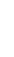
\includegraphics[max width=\linewidth, center]{external/whitespace-tikz/1cm.pdf}
\end{image}%
\item{}Resuelve el problema. Explica o muestra tu razonamiento.%
\begin{image}{0}{1}{0}{}%
\includegraphics[max width=\linewidth, center]{external/whitespace-tikz/6cm.pdf}
\end{image}%
\end{enumerate}
\end{project}
\end{document}